\begin{figure*}[t]
    \centering
    % trim={<left> <lower> <right> <upper>}
    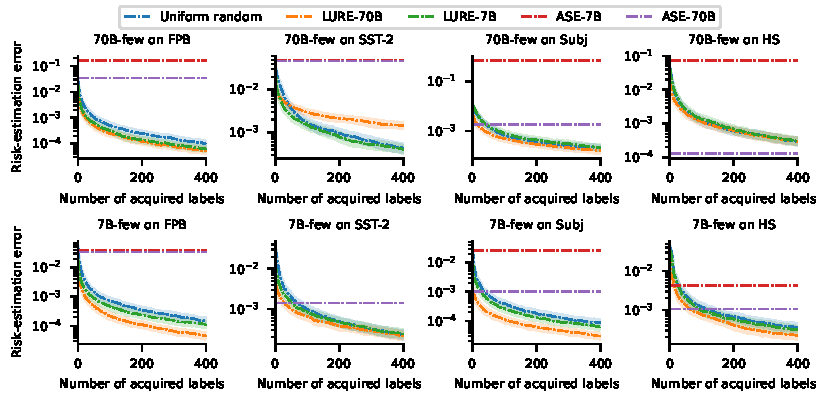
\includegraphics[width=0.95\linewidth,trim={0 5pt 0 0}]{
        figures/pdf/7b_70b_fewshot_lure_ase.pdf
    }
    \caption{
        Our sampling-based active testing (LURE) approach works more reliably than interpolation-based active testing (ASE) when using cheaply constructed surrogate models.
        In ASE the surrogate model not only guides data acquisition but also much more directly affects the risk estimate: the labels used to compute the expected loss of the target model are simulated from the surrogate model.
    }
    \label{fig:7b_70b_fewshot_lure_ase}
    \vspace{-8pt}
\end{figure*}